\chapter{Zadanie 5: Strojenie regulator�w}
\section{PID}
W tej cz??ci projektu laboratoryjnego dobierali?my parametry regulatora PID metod? eksperymentaln?. Poni?ej zosta? zamieszczony wykres wyj?cia obiektu dla dw�ch skok�w warto?ci zadanej z $36,5$ do $40$ oraz z $40$ do $38$. \

Pierwsze wykresy \ref{fig:lab05y} , \ref{fig:lab05u} oraz \ref{lab2eps} zosta?y wykonane w trakcie trwania laboratorium. Dla  \ref{fig:lab05y} , \ref{fig:lab05u} widzimy, ?e nastawy regulatora by?y nieodpowiednie. Regulator nie by? wstanie wysterowa? obiektu co odzwierciedla si? powolnym d??eniem do warto?ci zadanej oraz licznymi zawirowaniami przebieg�w sterowania i wyj?cia. Wykres \ref{lab2eps} jest ostatnim pomiarem jaki uda?o si? nam zebra? w trakcie trwania laboratorium. Z powodu braku czasu podczas laboratorium jest on w formacie $.eps$. Widzimy , ?e dla nowych nastaw uk?ad regulacji dzia?a? znacznie lepiej , charakteryzowa? si? ma?ym przeregulowaniem oraz wi?ksz? szybko?ci? zmian. Pr�bka oko?o 370 jest ostatni? jak? uda?o si? nam zebra? i na podstawie poprzednich pr�bek prognozujemy wyregulowanie obiektu. \\
\begin{figure}[tb]
	\centering
	\begin{tikzpicture}
	\begin{axis}[
	width=0.9\textwidth,
	height=0.6\textwidth,
	xmin=0,xmax=615,ymin=36,ymax=40.5,
	xlabel={$k$},
	ylabel={$Y(k)$},
	xtick={0,50,100,150,200,250,300,350,400,450,500,550,600},
	ytick={36,36.5,37,37.5,38,38.5,39,39.5,40,40.5},
	y tick label style={/pgf/number format/1000 sep=},
	]
	\addplot[blue,semithick] file {wykresy/pidy_0.5000_20.0000_5.0000.txt};
	\legend{$Y(k)$}
	\end{axis}
	\end{tikzpicture}
	\caption{Wyj?cie obiektu dla $K = 0,5 , T_i = 20, T_d = 5$}
	\label{fig:lab05y}
\end{figure}

\begin{figure}[tb]
	\centering
	\begin{tikzpicture}
	\begin{axis}[
	width=0.9\textwidth,
	height=0.6\textwidth,
	xmin=0,xmax=615,ymin=36,ymax=46,
	xlabel={$k$},
	ylabel={$U(k)$},
	xtick={0,50,100,150,200,250,300,350,400,450,500,550,600},
	ytick={36,37,38,39,40,41,42,43,44,45,46},
	y tick label style={/pgf/number format/1000 sep=},
	]
	\addplot[blue,semithick] file {wykresy/pidu_0.5000_20.0000_5.0000.txt};
	\legend{$U(k)$}
	\end{axis}
	\end{tikzpicture}
	\caption{Sterowanie obiektu dla $K = 0,5 , T_i = 20, T_d = 5$}
	\label{fig:lab05u}
\end{figure}

\begin{figure}[tb]
	\centering
	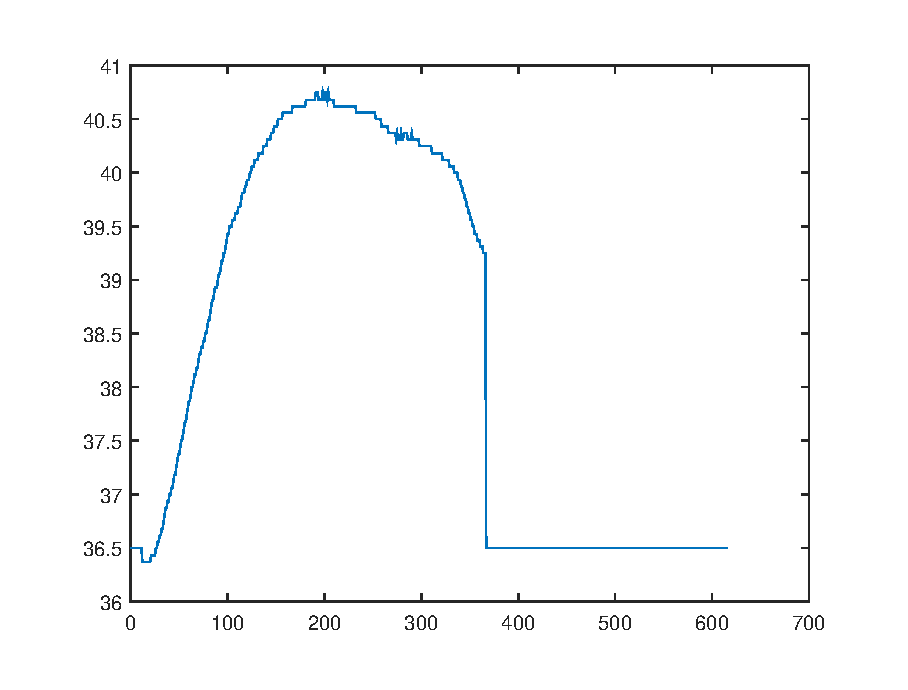
\includegraphics{wykresy/pid2_25_7.eps}
	\caption{Sterowanie obiektu dla $K = 2 , T_i = 25, T_d = 7$}
	\label{lab2eps}
\end{figure}

Dalsza cz??? projektu zosta?a wykonana na modelu obiektu w ?rodowisku domowym. \
Pierwsz? czynno?ci? jest zasymulowanie stanowiska dla ostatnich nastaw z laboratorium, aby sprawdzi? czy z grubsza pokrywaj? si? przebiegi \ref{domporownanie}.
Por�wnuj?c wykres \ref{lab2eps} wraz ze wspomnianym , zauwa?amy podobny z?b przy skoku warto?ci zadanej oraz podobne warto?ci przeregulowania. Sugurej?c si? tymi aspektami mo?na stwierdzi?, ?e model obiektu jest podobny do obiektu rzeczywistego, co ?wiadczy o poprawno?ci naszych przekszta?ce?. \\

\begin{figure}[tb]
	\centering
	\begin{tikzpicture}
	\begin{axis}[
	width=0.9\textwidth,
	height=0.6\textwidth,
	xmin=0,xmax=615,ymin=36,ymax=41,
	xlabel={$k$},
	ylabel={$Y(k)$},
	xtick={0,50,100,150,200,250,300,350,400,450,500,550,600},
	ytick={36,37,38,39,40,41},
	y tick label style={/pgf/number format/1000 sep=},
	]
	\addplot[blue,semithick] file {wykresy/pidy_2.0000_25.0000_7.0000.txt};
	\addplot[orange,semithick] file {wykresy/pidyzad_38.0000.txt};
	\legend{$Y(k)$,$Y_{zad}$}
	\end{axis}
	\end{tikzpicture}
	\caption{Sterowanie obiektu dla $K = 2, T_i = 25, T_d = 7$}
	\label{domporownanie}
\end{figure}


Na nast?pnych wykresach przedstawili?my wyniki symulacji dla r�?nych nastaw regulatora. Korzystamy z metody eksperymentalnej. Dob�r lepszych nastaw rozpoczynamy od dobrania parametru $K$. \\


\begin{figure}[tb]
	\centering
	\begin{tikzpicture}
	\begin{groupplot}[group style={group size=1 by 2,vertical sep={2 cm}},
	width=0.9\textwidth,height=0.3\textwidth]
	\nextgroupplot
	[
	xmin=0,xmax=615,ymin=0,ymax=100,
	xlabel={$k$},
	ylabel={$U$},
	xtick={0,50,100,150,200,250,300,350,400,450,500,550,600},
	ytick={0,10,20,30,40,50,60,70,80,90,100},
	y tick label style={/pgf/number format/1000 sep=},
	]
	\addplot[blue,semithick] file {wykresy/pidu_2.0000_Inf_0.0000.txt};
	\addplot[green,semithick] file {wykresy/pidu_3.0000_Inf_0.0000.txt};
	\addplot[magenta,semithick] file {wykresy/pidu_4.0000_Inf_0.0000.txt};
	\addplot[yellow,semithick] file {wykresy/pidu_5.0000_Inf_0.0000.txt};
	\nextgroupplot
	[
	xmin=0,xmax=615,ymin=36,ymax=41,
	xlabel={$k$},
	ylabel={$Y(k)$},
	xtick={0,50,100,150,200,250,300,350,400,450,500,550,600},
	ytick={36,37,38,39,40},
	y tick label style={/pgf/number format/1000 sep=},
	legend pos=south east,
	]
	\addplot[blue,semithick] file {wykresy/pidy_2.0000_Inf_0.0000.txt};
	\addplot[green,semithick] file {wykresy/pidy_3.0000_Inf_0.0000.txt};
	\addplot[magenta,semithick] file {wykresy/pidy_4.0000_Inf_0.0000.txt};
	\addplot[yellow,semithick] file {wykresy/pidy_5.0000_Inf_0.0000.txt};
	\addplot[orange,semithick] file {wykresy/pidyzad_38.0000.txt};
	\legend{$K=2$,$K=3$,$K=4$,$K=5$,$Y^{zad}$}
	\end{groupplot}
	\end{tikzpicture}
	\caption{Dob�r parametru K}
	\label{doborK}
\end{figure}

Zgodnie z rysunkiem \ref{doborK} mo?na zauwa?y?, ?e dla $K>3$ zaczyna wyst?powa? przeregulowanie oraz szybko?? regulacji jest coraz mniejsza. W dalszych rozwa?aniach potraktowali?my jako warto?? prawid?ow? $K=4$ , gdy? zmiany s? nik?e , a wi?kszy cz?on proporcjonalny pozwoli nam zwi?kszy? "agresywno??" regulatora. \

\begin{figure}[tb]
	\centering
	\begin{tikzpicture}
	\begin{groupplot}[group style={group size=1 by 2,vertical sep={2 cm}},
	width=0.9\textwidth,height=0.3\textwidth]
	\nextgroupplot
	[
	xmin=0,xmax=615,ymin=0,ymax=100,
	xlabel={$k$},
	ylabel={$U$},
	xtick={0,50,100,150,200,250,300,350,400,450,500,550,600},
	ytick={0,10,20,30,40,50,60,70,80,90,100},
	y tick label style={/pgf/number format/1000 sep=},
	]
	\addplot[blue,semithick] file {wykresy/pidu_4.0000_90.0000_0.0000.txt};
	\addplot[green,semithick] file {wykresy/pidu_4.0000_80.0000_0.0000.txt};
	\addplot[magenta,semithick] file {wykresy/pidu_4.0000_70.0000_0.0000.txt};
	\nextgroupplot
	[
	xmin=0,xmax=615,ymin=36,ymax=41,
	xlabel={$k$},
	ylabel={$Y(k)$},
	xtick={0,50,100,150,200,250,300,350,400,450,500,550,600},
	ytick={36,37,38,39,40},
	y tick label style={/pgf/number format/1000 sep=},
	legend pos=south east,
	]
	\addplot[blue,semithick] file {wykresy/pidy_4.0000_90.0000_0.0000.txt};
	\addplot[green,semithick] file {wykresy/pidy_4.0000_80.0000_0.0000.txt};
	\addplot[magenta,semithick] file {wykresy/pidy_4.0000_70.0000_0.0000.txt};
	\addplot[orange,semithick] file {wykresy/pidyzad_38.0000.txt};
	\legend{$T_i=90$,$T_i=80$,$T_i=70$,$Y^{zad}$}
	\end{groupplot}
	\end{tikzpicture}
	\caption{Dob�r parametru $T_i$}
	\label{doborTi}
\end{figure}

Nast?pnym dobranym parametrem jest $T_i$ \ref{doborTi}. Na podstawie utworzonych wykres�w jednoznacznie mo?na stwierdzi?, ?e najlepszy przebieg jest osi?gany dla warto?ci $T_i = 80 $. Dla warto?ci $T_i = 90$ uk?ad mimo i? znajduje si? blisko warto?ci zadanej osi?ga j? bardzo wolno, a dla $T_i = 70$ wyst?puje znaczne przeregulowanie. \

\begin{figure}[tb]
	\centering
	\begin{tikzpicture}
	\begin{groupplot}[group style={group size=1 by 2,vertical sep={2 cm}},
	width=0.9\textwidth,height=0.3\textwidth]
	\nextgroupplot
	[
	xmin=0,xmax=615,ymin=0,ymax=100,
	xlabel={$k$},
	ylabel={$U$},
	xtick={0,50,100,150,200,250,300,350,400,450,500,550,600},
	ytick={0,10,20,30,40,50,60,70,80,90,100},
	y tick label style={/pgf/number format/1000 sep=},
	]
	\addplot[blue,semithick] file {wykresy/pidu_4.0000_80.0000_0.0000.txt};
	\addplot[green,semithick] file {wykresy/pidu_4.0000_80.0000_1.5000.txt};
	\addplot[magenta,semithick] file {wykresy/pidu_4.0000_80.0000_3.0000.txt};
	\addplot[red,semithick] file {wykresy/pidy_4.0000_80.0000_4.0000.txt};
	\nextgroupplot
	[
	xmin=0,xmax=615,ymin=36,ymax=41,
	xlabel={$k$},
	ylabel={$Y(k)$},
	xtick={0,50,100,150,200,250,300,350,400,450,500,550,600},
	ytick={36,37,38,39,40},
	y tick label style={/pgf/number format/1000 sep=},
	legend pos=south east,
	]
	\addplot[blue,semithick] file {wykresy/pidy_4.0000_80.0000_0.0000.txt};
	\addplot[green,semithick] file {wykresy/pidy_4.0000_80.0000_1.5000.txt};
	\addplot[magenta,semithick] file {wykresy/pidy_4.0000_80.0000_3.0000.txt};
	\addplot[red,semithick] file {wykresy/pidy_4.0000_80.0000_4.0000.txt};
	\addplot[orange,semithick] file {wykresy/pidyzad_38.0000.txt};
	\legend{$T_d=0$,$T_d=1.5$,$T_d=3$,$T_d=4$,$Y^{zad}$}
	\end{groupplot}
	\end{tikzpicture}
	\caption{Dob�r parametru $T_d$}
	\label{doborTd}
\end{figure}

Ostatnim dobranym parametrem jest $T_d$ \ref{doborTd}. Po zmianie z zera na wi?ksze warto?ci okazuje si?, ?e mimo mniejszego przeregulowania obiekt potrzebuje wi?cej czasu na osi?gni?cie dok?adnej warto?ci zadanej, jednak?e po przeanalizowaniu wskanika regulacji $E$ :\\
\begin{itemize}
	\item $T_d = 0$ - $E = 282.5235$ 
	\item $T_d = 0$ - $E = 267.5491$ 
	\item $T_d = 0$ - $E = 254.5283$ 
	\item $T_d = 0$ - $E = 402.4649$ 		 
\end{itemize}\

?atwo zauwa?y?, ?e $T_d = 3$ jest najlepsz? warto?ci?.

Najlepsze przebiegi dla naszego obiektu uzyskali?my stosuj?c nast?puj?ce nastawy $K_p = 4 , T_i = 80 , T_d = 3$ , gdzie wskaznik jako?ci $E = 254.5283 $.
